\documentclass[11pt]{article}
\usepackage[T1]{fontenc}
\usepackage{lmodern}
\usepackage[letterpaper, margin=15mm]{geometry}
\usepackage{xcolor}
\usepackage{tikz}
\usepackage[skins]{tcolorbox}
\usepackage{enumitem}
\usepackage{array}

% Cheerful colours. Change them to your school colours.
\definecolor{sky}{HTML}{3A86FF}
\definecolor{sun}{HTML}{FFBE0B}
\definecolor{berry}{HTML}{FF006E}
\definecolor{leaf}{HTML}{38B000}
\definecolor{grape}{HTML}{8338EC}

\renewcommand{\familydefault}{\sfdefault}
\pagestyle{empty}
\setlength{\parindent}{0pt}
\setlength{\parskip}{3pt}
\setlist{leftmargin=1.2em, itemsep=1pt, topsep=2pt}

% A rounded box with a tab title. Usage: \begin{bubble}{colour}{Title} ... \end{bubble}
\newtcolorbox{bubble}[2]{enhanced, colback=#1!8, colframe=#1, boxrule=1.2pt, arc=4mm,
  left=3mm, right=3mm, top=4mm, bottom=2mm, before skip=0pt, after skip=4mm,
  attach boxed title to top left={xshift=4mm, yshift=-3mm},
  boxed title style={colback=#1, colframe=#1, arc=2mm}, fonttitle=\bfseries, title=#2}

% A tick box for the reminders checklist.
\newcommand{\checkbox}{\raisebox{-1pt}{\tikz\draw[thick, grape, rounded corners=1pt] (0,0) rectangle (9pt,9pt);}\ }

\begin{document}

% Header: class name, teacher and month.
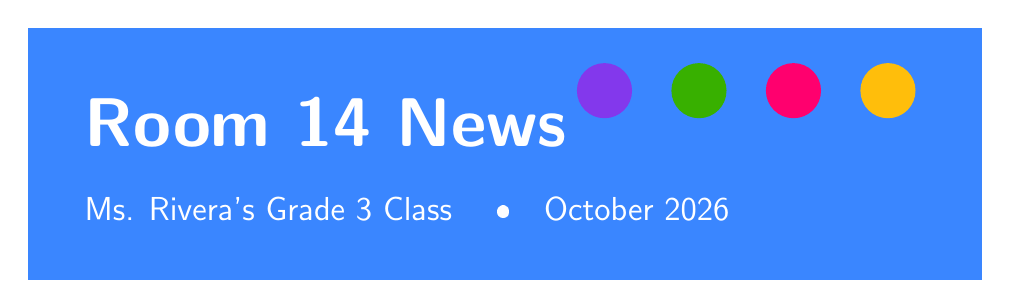
\begin{tikzpicture}
  \fill[sky] (0,0) rectangle (\textwidth, 3.2cm);
  \foreach \x/\c in {1.2/sun, 2.4/berry, 3.6/leaf, 4.8/grape} {
    \fill[\c] (\textwidth-\x cm, 2.4) circle (0.35);
  }
  \node[anchor=west, text=white, font=\bfseries\fontsize{30}{34}\selectfont] at (0.6,2.0) {Room 14 News};
  \node[anchor=west, text=white, font=\large] at (0.6,0.9) {Ms. Rivera's Grade 3 Class \quad \textbullet\quad October 2026};
\end{tikzpicture}

\vspace{5mm}

\begin{minipage}[t]{0.58\textwidth}
  \vspace{0pt}
  \begin{bubble}{sky}{Hello families!}
    What a wonderful start to autumn. Our class has settled into new routines, and I am so proud of how kindly everyone works together.
    This month we will explore the water cycle, practise times tables and start our first chapter book together.
    \par\medskip
    Thank you for the donations of tissues and glue sticks!
    \par\hfill\emph{Ms. Rivera}
  \end{bubble}

  \begin{bubble}{leaf}{What we are learning}
    \begin{tabular}{@{}>{\bfseries}p{0.22\linewidth}p{0.7\linewidth}@{}}
      Reading & \emph{The Lighthouse Mouse}, chapters 1 to 6 \\
      Maths & Times tables 2, 5 and 10 \\
      Science & The water cycle and weather \\
      Art & Leaf printing and colour mixing \\
    \end{tabular}
  \end{bubble}

  \begin{bubble}{berry}{Student corner}
    \begin{minipage}[t]{0.36\linewidth}
      \vspace{0pt}
      \tikz\node[draw=berry, dashed, minimum width=\linewidth, minimum height=2.8cm, font=\small, align=center]{Image\\placeholder};
    \end{minipage}\hfill
    \begin{minipage}[t]{0.6\linewidth}
      \vspace{0pt}
      \textbf{Star of the week: Jonah}\\
      Jonah helped a new classmate find their way around school all week. He loves dinosaurs and drawing maps.
    \end{minipage}
  \end{bubble}

  \begin{bubble}{grape}{Try this at home}
    \begin{itemize}
      \item Read together for 15 minutes each evening.
      \item Count coins or snacks in groups of 2, 5 and 10.
      \item Watch the sky and keep a one week weather diary.
      \item Ask your child to explain one new thing they learned today.
    \end{itemize}
  \end{bubble}

  \begin{bubble}{sun}{Classroom wish list}
    Old magazines for collage, a few board games and paper towel tubes for our science projects. Thank you!
  \end{bubble}
\end{minipage}\hfill
\begin{minipage}[t]{0.38\textwidth}
  \vspace{0pt}
  \begin{bubble}{sun}{Important dates}
    \renewcommand{\arraystretch}{1.25}
    \begin{tabular}{@{}>{\bfseries}l l@{}}
      Oct 6 & Library day \\
      Oct 13 & Picture day \\
      Oct 17 & No school \\
      Oct 22 & Parent meetings \\
      Oct 30 & Costume parade \\
    \end{tabular}
  \end{bubble}

  \begin{bubble}{grape}{Reminders}
    \checkbox Return reading logs each Friday\\
    \checkbox Label jackets and water bottles\\
    \checkbox Sign the field trip form\\
    \checkbox Pack a healthy snack
  \end{bubble}

  \begin{bubble}{leaf}{Word of the month}
    \centering
    {\Large\bfseries evaporate}\par
    \small to turn from a liquid into a gas
  \end{bubble}

  \begin{bubble}{sky}{Contact me}
    \small
    Email: rivera@school.example\\
    Phone: 000 000 0000\\
    I reply within one school day.
  \end{bubble}
\end{minipage}

\vfill
\begin{tcolorbox}[colback=sun!25, colframe=sun!25, arc=3mm, halign=center]
  \bfseries Thought for the month: Be the reason someone smiles today.
\end{tcolorbox}

\end{document}
